\section{Hintergrund und Verwandte Arbeiten}

\subsection{Angry Birds als Herausforderung im Bereich Künstliche Intelligenz}
In physikbasierten Simulationsspielen wie Angry Birds ist die gesamte Spielwelt typischerweise parametrisiert. So sind beispielsweise alle physischen Parameter, wie die Masse, die Reibung, die Dichte von Objekten und die Gravität sowie alle Objekttypen und deren Eigenschaften und Lage intern bekannt. Jede gewählte Aktion kann deshalb mit einem zugrundeliegenden Physik-Simulator sehr realgetreu nachgebildet werden. Einfache Aktionen können wie folgt beschrieben werden: der Spieler kann erstens entscheiden an welchem Punkt <x,y> der Vogel aus der Schleuder gelassen werden soll und zweitens wann während des Flugs die Superkraft des Vogels aktiviert werden soll. In der Praxis ergibt dies eine sehr große Anzahl an möglichen Aktionen. Während des Spielens gilt ein Level immer dann als gelöst, wenn eine Reihe von Aktionen zu einem Spielstand führt, der bestimmte Siegbedingungen erfüllt.\\
Aus dem einfachen Spiel und den einfachen Aktionen resultiert, dass auch kleine Kinder das Spiel schon erfolgreich durchspielen können. Die Herausforderung des Wettbewerbs besteht also darin einen intelligenten Agenten zu bauen, der neue Level genauso gut oder sogar erfolgreicher spielen kann als die besten menschlichen Spieler. Im Vergleich zu scheinbar harten Spielen wie z.B. Schach klingt dies nach einer relativ einfachen Aufgabe, allerdings müssen einige Herausforderungen gemeistert werden. Unter der Annahme, dass alle Parameter der Spielwelt bekannt und parametrisiert sind, könnten Aktionen und deren Folgeaktionen solange simulieret werden bis der Siegzustand erreicht ist. Wenn die Handlungen dann noch intelligent ausgewählt werden, kann dies zu einer erfolgreichen Lösungsstrategie führen.\\
Hier liegt aber das Hauptproblem physikbasierter Simulationsspiele: das Ergebnis von Aktionen ist immer erst dann bekannt, wenn diese simuliert wird, was wiederum bedeutet, dass auch alle dafür benötigten Parameter bekannt sein müssen. Es liegt also eine andere Grundlage vor als bei Spielen wie Schach, in denen die Ergebnisse jeder Aktion schon im Voraus bekannt sind. Hinzu kommt, dass sich die Spielwelt nach jedem Schuss enorm verändert. Dies erfordert also präzise Vorhersagen oder Annäherungen an die resultierenden Konsequenten, um eine Strategie aus Aktionen entwickeln zu können. Die Kombination aus einem potentiell unendlichen Aktionsraum und dem möglichen Mangel an Informationen über alle Parameter stellt hinsichtlich des Treffens von Vorhersagen eine der größten Herausforderungen dar. Für den Menschen eine relativ einfache Aufgabe, allerdings ist das Kombinieren in unbekannten Umgebungen noch immer eine Forschungsfrage.\\
Die Forschung an physikbasierten Simulationsspielen wie Angry Birds ist deshalb so wichtig, weil die gleichen Probleme auch noch für AI-Systeme gelöst werden müssen, damit diese erfolgreich mit der physischen Welt interagieren können. Während Menschen diese Fähigkeit einfach haben und ständig einsetzen, ist aus Sicht von AI noch nicht das ganze Potential ausgeschöpft. Der IJCAI 2017 Angry Birds AI Wettbewerb bietet dazu eine geeignete Plattform an, um diese Herausforderungen und neuen Fähigkeiten in einer vereinfachten und kontrollierten Umgebung zu testen und zu entwickeln.

\subsection{Verwandte Arbeiten}
2013 veröffentlichte [Calimeri et al., 2013] den Artikel "AngryHEX: an Artificial Player for Angry Birds Based on Declarative Knowledge Bases". Diese Arbeit präsentiert ein gemeinsames Projekt der Universität von Kalabrien (UniCal) und der TU Wien, mit dem Ziel, einen intelligenten Agenten zu entwickeln, der am 2013 Angry Birds AI Wettbewerb teilnimmt. AngryHEX, so die Autoren, basiert auf einer Programmierung mit Hilfe von ASP (Answer Set Programming). Die grundlegende Spielsoftware, die von den Veranstaltern zur Verfügung gestellt wird, wurde ebenfalls verwendet. Diese wurde allerdings noch durch eine Erweiterung modifiziert, die Informationen über die aktuelle Szene in logische Behauptungen kodiert.\\
[Ferreira et al., 2013] beschreibt die Aufgabe des Projekts wie folgt. Laut den Autoren ist das Ziel einen autonomen Agenten zu entwickeln, der in der Lage ist, ohne menschliches Eingreifen [Angry Birds] zu spielen. Dabei ist dieser in der Lage ist seine Umgebung zu betrachten und mit einzubeziehen. Außerdem ist der Agent in der das beste Objekt als Ziel auszuwählen. Der Artikel beschreibt weiterhin die Entwicklung eines intelligenten Agenten namens FEI2, der für einen Wettbewerb 2012 entwickelt wurde. Der Schwerpunkt, so [Ferreira et al., 2013] weiter lag dabei auf der Auswahl des bestmöglichen Ziels. Zudem wurden für die Entwicklung drei Konzepte kombiniert. Einmal lag die Konzentration auf der räumlichen Darstellung der einzelnen Objekte, weil die Positionen der Objekte und die Lagebeziehungen derer untereinander wichtig seien. Die Autoren schreiben weiter: "The second concept is that of Utility Function, which allows the agent to represent preferences for the options that are given to it". Das zweite Konzept gibt dem Agenten also die Funktion Präferenzen für ein Zielobjekt abzugeben, dies ist wichtig bei der Entscheidungsfindung. Schließlich wurde als letztes Konzept Schlussfolgern unter Unsicherheit verwendet.\\
Mihai Polceanu und Cedric Buche konzentrieren sich in ihrem Artikel auf einen bestimmten Bereich für die Ausarbeitung eines intelligenten Agenten. Sie schreiben über verschiedene Entscheidungsmechanismen. Dabei liegt der Fokus vor allem auf der Erwartungsfähigkeit des Menschen und seiner Fähigkeit sich anzupassen, während diese interagieren. Da dieser Bereich auch für den intelligenten Agenten erarbeitet und implementiert werden soll, ist auch dieser Artikel sehr hilfreich bei der Ausarbeitung.

\subsection{Der IJCAI 2017 Angry Birds AI Wettbewerb}
Im Zuge des Wettbewerbs sollen die Fähigkeiten des entwickelten intelligenten Agenten für Angry Birds getestet werden. Dazu werden von Seiten der Veranstalter eine Vielzahl von Level angeboten, um in einer vereinfachten und kontrollierten Umgebung die Enticklung und Erprobung des Agenten voranzutreiben. Langfristig gesehen, soll der Wettbewerb beim Aufbau eines AI-Agenten unterstützen, der für ihn unbekannte Level besser spielen kann als die besten menschlichen Angry Birds Spieler.\\
Wie oben bereits beschrieben, ist dies ein sehr schwieriges Problem, da es erfordert, dass der Agent Handlungen vorhersagen kann, ohne aber die Spielwelt komplett zu kennen. Zusätzlich muss eine gute Handlungsauswahl implementiert werden.\\
Zu beachten ist, dass Level in beliebiger Reihenfolge gespielt und auch so oft wie nötig wiederholt werden können. Die Agenten werden danach anhand der insgesamt erreichten Punkte bewertet. Während des Wettbewerbs „Mensch gegen Maschine“ wird dann getestet, ob der Agent besser ist als menschliche Spieler. Folgende Probleme müssen dafür effizient gelöst werden:

\begin{itemize}
\item Erkennen und klassifizieren bekannter und unbekannter Objekte,
\item Erlernen von Eigenschaften der (unbekannten) Objekte und der Spielwelt,
\item Vorhersage des Handlungsergebnisses,
\item Auswahl guter Aktionen in vorgegebenen Situationen und
\item Planung einer erfolgreichen Aktionssequenz sowie
\item  der Reihenfolge in der Level gespielt werden sollen.
\end{itemize}

Gespielt wird die Google Chrome Version von Angry Birds, die unter chrome.angrybirds.com öffentlich zugänglich ist. Der zur Verfügung gestellte Wettkampfserver verbindet sich dadurch mit der zuvor eingerichteten Chrome Browser Erweiterung, durch die es möglich ist Screenshots des Spiels während der Laufzeit aufzunehmen. Außerdem können darüber auch die verschiedenen Aktionen per Mausklick ausgeführt werden. Teilnehmende Agenten, die sich auf verschiedenen Clients laufen müssen, können nur über ein festes Kommunikationsprotokoll mit dem Server interagieren. Dies ermöglicht dem Agenten das Anfordern von Screenshots, Aktionen und anderen Befehlen vom Server und das Ausführen dieser im Live-Spiel. U.a. kann auch der aktuelle Highscore jederzeit vom Server abgerufen werden. Den Agenten wird so die gleiche Information wie dem Menschen zur Verfügung gestellt. Die genaue Lage oder Parameter von Objekten bleiben allerdings trotzdem unbekannt.\\
Um das Problem zu vereinfachen und sich ganz auf die Entwicklung des Agenten zu konzentrieren, verwenden wir die von den Organisatoren zur Verfügung gestellte grundlegende Spielsoftware. Das Grundgerüst dieser Software besteht aus drei Komponenten:

\begin{itemize}
\item Computer-Vision-Komponente (engl.: computer vision component), die einen Ausschnitt des Videospiels analysieren kann und den Ort, die Kategorie und die Begrenzungsbox (Bounding Box) alles relevanten Objekte sowie den Spielstand indentifiziert
\item Trajektorien-Komponente (trajectory component), die Trajektorien von Vögeln berechnet und berechnet wohin man schießen muss, um ein bestimmtes Objekte oder einen bestimmten Ort zu treffen
\item -	Spielkomponente, die Aktionen ausführt und Screenshots erfasst.
\end{itemize}

\subsection{Meta-Strategie des Agenten "BamBird" 2017}
Für die Teilnahme am Wettbewerb hat sich das gesamte Projektteam in insgesamt vier Untergruppen geteilt. Jede Gruppe übernahm eine andere Aufgabe für die Entwicklung des Agenten. Die Aufteilung war wie folgt: Physiksimulation, Entwicklung neuer Schuss-Strategien, Anpassung des Schussmoduls und Meta-Strategie.\\
Das Zusammenspiel der Komponenten ist in folgendem Diagramm dargestellt:

\begin{figure} [h]
	\begin{center}
		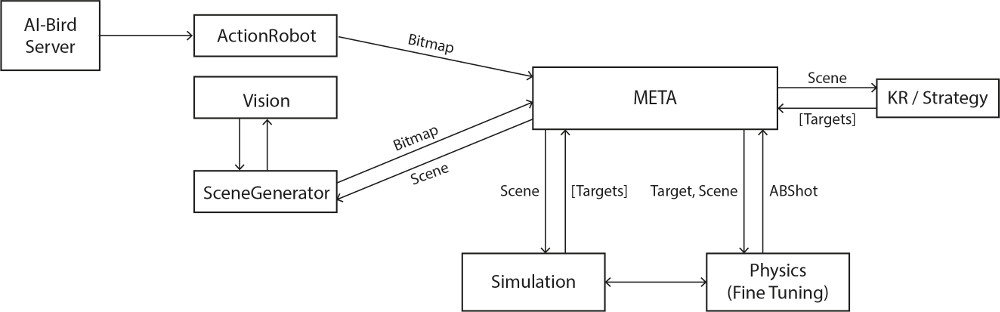
\includegraphics[width=1\textwidth]{ablaufdiagramm1}
		\caption{Wechselspiel der einzelnen Komponenten des Wettbewerbs.}
	\end{center}
\end{figure}

In diesem Bericht soll insbesondere auf die Arbeit des Meta-Teams eingegangen werden. Diese übergreift alle anderen Komponenten und führt diese zusammen, die Gruppe "Meta" ist also eine Art Schnittstelle für die anderen Gruppen.\\
Wir haben uns insbesondere folgenden Arbeitsfeldern angenommen. Als Erstes haben wir uns mit der Auswahl der verschiedenen Level während des Spiels beschäftigt. So nehmen wir Einfluss auf den Spielfluss und entscheiden in welcher Reihenfolge und wie oft die einzelnen Level gespielt werden sollen.
Eine weitere wichtige Aufgabe ist es, die richtigen Aktionen auszuwählen. Wir haben uns in dieser Hinsicht auf die Auswahl der Schüsse spezialisiert. Aus einer Liste, die wir von der Strategie-Gruppe erhalten, wählen wir, den als besten markierten Schuss aus. Zur Vorhersage einer guten Handlung haben wir uns des weiteren eine Form der Evaluation einzelner Schüsse überlegt, um besonders gute Schüsse zu kennzeichnen und diese in ähnlichen Situationen wieder anzuwenden.
Alle Informationen werden zu jedem einzelnen Schuss in einer Datenbank gespeichert, die wir implementiert haben.\\
Genaue Informationen über den Vorgang unserer Implementierung werden im folgenden Kapitel näher ausgeführt.